\documentclass[letterpaper,12pt]{article}

%\usepackage{ucs}
%\usepackage[utf8x]{inputenc}
\usepackage{amsmath}
\usepackage{amsfonts}
\usepackage{amssymb}
\usepackage{graphicx}
%\usepackage[canadian]{babel}
\usepackage[margin=1in]{geometry}
\newcommand{\R}{\mathbb{R}}
\renewcommand{\i}{\mathbf{i}}
\renewcommand{\j}{\mathbf{j}}
\renewcommand{\k}{\mathbf{k}}

\title{Practice for Quiz 8\\Math 2580\\Spring 2016}
\author{Sean Fitzpatrick}
\date{February 4th, 2016}

\begin{document}
 \maketitle

If you can answer the following problems, you should be well-prepared for Quiz 8:



\begin{enumerate}
 \item Find the critical points of the following functions:
\begin{enumerate}
 \item $f(x,y) = x^2y-xy^2$
 \item $f(x,y) = x^2+y^2-2xy$
 \item $f(x,y) = 2(x^2+y^2)e^{-x^2-y^2}$
\end{enumerate}
 \item Consider the function $f(x,y)=xy+5y$, defined on the disc $D=\{(x,y) | x^2+y^2\leq 4\}$.
\begin{enumerate}
 \item Find any critical points of $f$ that are contained within $D$.
 \item Recall that the circle $x^2+y^2=4$ can be parameterized using $r(t) = (2\cos t, 2\sin t)$, with $t\in [0,2\pi]$. Find any critical points of the one-variable function $g(t) = f(2\cos(t),2\sin(t))$ on the interval $[0,2\pi]$. (This is a Calc I question.)
 \item Using your answers from (a) and (b), determine the absolute maximum and minimum of $f$ on the disc $D$.
\end{enumerate}

{\bf Continue to the next page for more fun...}

\pagebreak
\item In the diagram on below, I've plotted several level curves for the function $f(x,y)=x^2y-xy^2$, along with the parabola $y=x^2$. The marked point $(a,b)$ is the intersection of the curve $x^2y-xy^2=1$ (in yellow), with the parabola $y=x^2$. Suppose we want to find the maximum value of $f(x,y)$ subject to the constraint $y=x^2$.
\begin{enumerate}
 \item Explain why the maximum cannot occur at the point $(a,b)$.
 \item Indicate a point on the graph where the maximum {\em might} occur.
\end{enumerate}

\begin{center}
 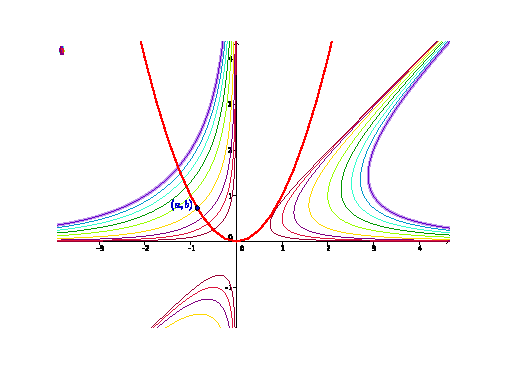
\includegraphics[width=\textwidth]{Q8-3}
\end{center}
\item Make sure you can do the problems in Question 1. Your quiz will be one of those.
\end{enumerate}

\end{document}
 
